\documentclass[11pt, a4paper, french]{article}
\setlength{\parindent}{0pt}

% -----------------------------------------------------------------------
% --- PACKAGES ---
% -----------------------------------------------------------------------
\usepackage[utf8]{inputenc}
\usepackage[T1]{fontenc}
\usepackage{ae, pslatex}
\usepackage[french]{babel}
\usepackage{fancyhdr}
\usepackage{lastpage}
\usepackage{vmargin}
\usepackage{enumitem}
\usepackage{multirow}
\usepackage{graphicx}


% -----------------------------------------------------------------------
% --- MARGES ---
% -----------------------------------------------------------------------
\setpapersize{A4}
\setmarginsrb{60pt}{50pt}{60pt}{25pt}{15pt}{25pt}{15pt}{30pt}


% -----------------------------------------------------------------------
% --- EN-TETE ET PIED DE PAGE ---
% -----------------------------------------------------------------------
\pagestyle{fancy}
\fancyhf{} % Supprime les entetes et pieds de page existants

\fancyhead[L]{Projet de semestre\\}
\fancyhead[R]{IL - TIC - HEIG-VD \\ Printemps 2017}
\fancyfoot[L]{E. Ransome, G. Milani, S. Kirushnapillai, M. Spierer}
\fancyfoot[R]{\thepage{}}


\title{Editeur d'images GEMMS \\ Cahier des charges}
\author{E. Ransome, G. Milani, S. Kirushnapillai, M. Spierer}
\date{Mars 2017}

% ***********************************************************************
% *** DOCUMENT PRINCIPAL ***
% ***********************************************************************
\begin{document}
	\maketitle
	\thispagestyle{empty}
	\tableofcontents
	\pagebreak

	\section{Description}
		Dans le cadre du projet de semestre de deuxième année, nous allons développer un éditeur d'image simple et intuitif. L'application permettra d'ajouter du texte, dessiner à l'aide d'outils divers, ou d'appliquer des filtres sur des images. Il permettra également les fonctionnalités de base d'un éditeur d'image, à savoir, redimensionner, rogner et transformer une image. \\
		
		Pour ce faire, il sera possible de créer, d'ouvrir et de sauvegarder un document. Les documents utiliseront la notion de calque afin de gérer l'ensemble des objets tel que les textes, images, etc. \\
		
		L’interface permettra de redimensionner l’espace de travail à la taille voulue et de se déplacer de manière aisée à l’intérieur de celui-ci. \\
		
		Pour finir l’application sera développée à l’aide de JavaFX et supportera les format jpg, png, bmp et gif.
	
	\section{Objectifs et Fonctionnalités}

		L'objectif principal est de développer une application simple et intuitif. Par conséquent, nous ne voulons pas ressembler aux applications lourdes telles que Photoshop ou Gimp qui proposent énormément de fonctionnalités. En effet, ces logiciels demandent beaucoup de temps d'apprentissage et par conséquent, ils ne sont pas facile d'accès. 
		 
		\subsection{Fonctionnalités de base}
			
			Ci-dessous les fonctionnalités à réaliser au terme du projet.\\
			
			\textbf{Création de document}
			\begin{itemize}[label=\textbullet]
				\item Créer un document vide.
				\item Gestion des calques.
				\item Sauvegarde du documenette section pésentet.
				\item Exporter aux formats png, jpg, bmp et gif.
				\item Insérer une image dans un document. \\
			\end{itemize}
		
			\textbf{Transformations d'objets}
			\begin{itemize}[label=\textbullet]
				\item Redimensionner, Pivoter, Déplacer un élément du dessin.
				\item Symétrie horizontale / verticale des éléments du dessin.
				\item Affichage de repères d'alignement automatiques simples.\\
			\end{itemize}
		
			\textbf{Fonctionnalités de dessin}
			\begin{itemize}[label=\textbullet]
				\item Pinceau
					\begin{itemize}[label=\textbullet]
						\item Choisir la taille du pinceau.
						\item Choisir la couleur du pinceau.
					\end{itemize}
				\item Gomme
					\begin{itemize}[label=\textbullet]
						\item Choisir la taille de la gomme.
					\end{itemize}
				\item Pipette
					\begin{itemize}[label=\textbullet]
						\item Récupération de couleur sur un emplacement. \\
					\end{itemize}
			\end{itemize}
		
			\textbf{Historique}
			\begin{itemize}[label=\textbullet]
				\item Annuler une action.
				\item Réitérer une action.
				\item Parcours visuel de l'historique. \\
			\end{itemize}
		
			\textbf{Fonctionnalités colorimétrique}
			\begin{itemize}[label=\textbullet]
				\item Application de filtres prédéfinis.
				\item Modification de contraste.
				\item Modification de luminosité.
			\end{itemize}
	
			\textbf{Fonctionnalités de sélection}
			\begin{itemize}[label=\textbullet]
				\item Sélection manuelle d’une zone de pixels.
				\item Copier, coller, modifier, supprimer une sélection. \\
			\end{itemize}
	
			\textbf{Fonctionnalités texte}
			\begin{itemize}[label=\textbullet]
				\item Ajout d’éléments textes.
				\item Choix de couleur.
				\item Choix de police.
				\item Choix de taille. \\
			\end{itemize}
	
			\textbf{Cadre de travail}
			\begin{itemize}[label=\textbullet]
				\item Interface de l’application.
				\item Navigation dans l’espace de travail.
				\begin{itemize}[label=\textbullet]
					\item Déplacement.
					\item Zoom.
				\end{itemize}
				\item Gestion des couleurs.
				\item Raccourcis claviers.
				\item Modifier la taille de l’espace de travail et du document.
				\item Rogner le document.
				\item Copier-Coller d’éléments de dessin. \\
			\end{itemize}
		
			\textbf{Fonctionnalités diverses}
			\begin{itemize}[label=\textbullet]
				\item Modifier la taille de l’espace de travail et du document.
				\item Rogner le document.
				\item Copier-Coller d’éléments de dessin. \\
			\end{itemize}

		
		\subsection {Fonctionnalités optionnelles}
		
		Ci-dessous, les fonctionnalités optionnelles à réaliser dans le future.\\
		
			\textbf{Fonctionnalités diverses}
			\begin{itemize}[label=\textbullet]
				\item Bibliothèque personnelle d’image.
				\item Différents catalogues d’images.
				\item Possibilité de lister ces catalogues dans l’application.
				\item Possibilité d’importer ces images dans des documents. \\
			\end{itemize}
		
			\textbf{Paramétrage de l’application}
			\begin{itemize}[label=\textbullet]
				\item Raccourcis claviers.
				\item Position du menu d’outils.
				\item Options de nouveau document.
				\item Taille prédéfinie du document.
				\item Configuration des raccourcis. \\
			\end{itemize}
			
	
	\pagebreak
	\section{Maquettes}
	
		Cette section présente un premier aperçu du programme. En haut, nous avons une barre de raccourci permettant de créer un nouveau document, sauvegarder, etc. A gauche, nous avons les différents outils disponibles de l'éditeur. Puis, au milieu, nous avons le cadre de travail. Et enfin à droite, nous avons la liste des objets et l'historique des actions effectuées.\\
	
		\begin{figure}[h!] 
			\centering
			\graphicspath{{Mockups/}}
			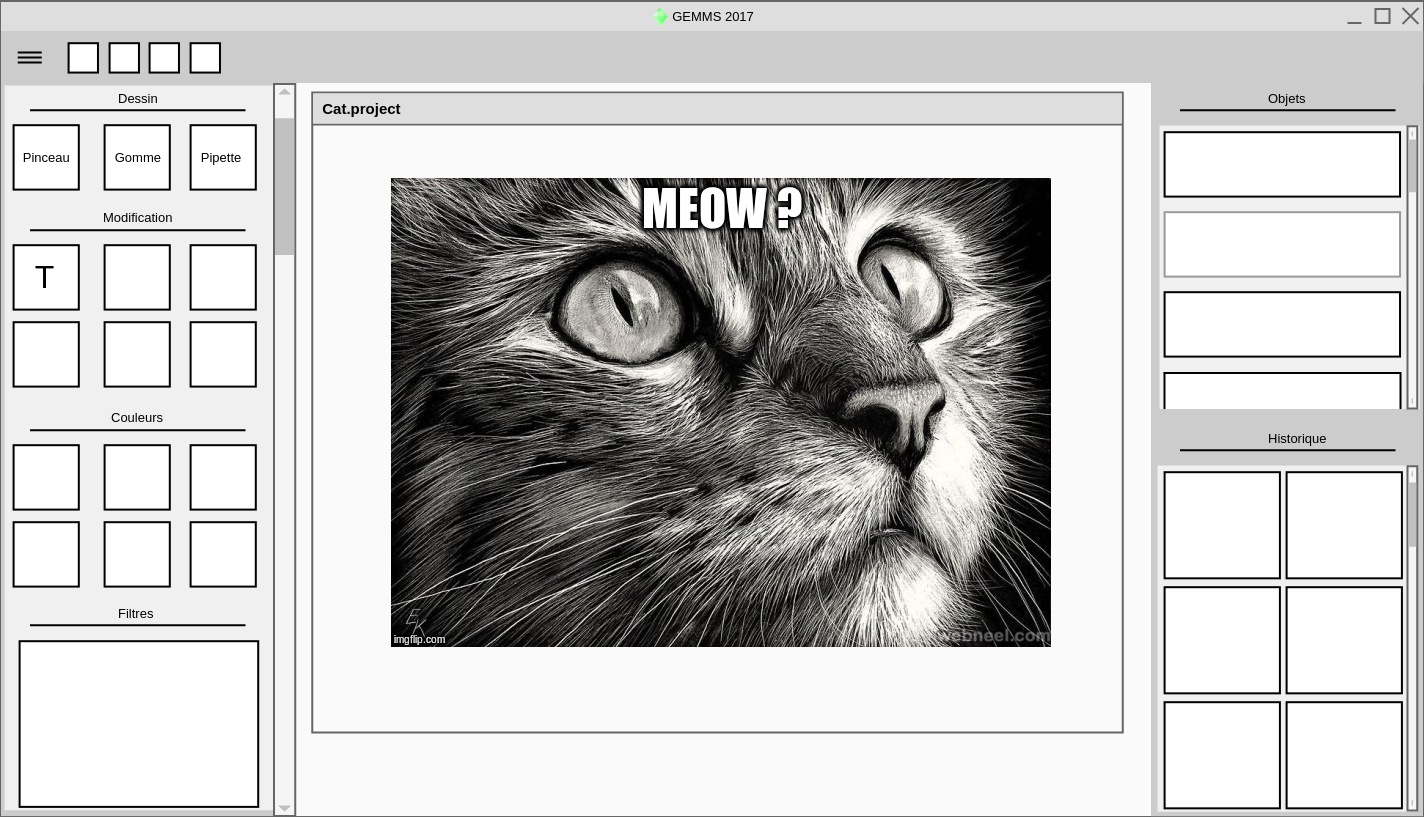
\includegraphics[scale=0.3]{home_page.png}
			\caption{\label{étiquette} Interface de base}
		\end{figure}
	
		\begin{figure}[h!] 
			\centering
			\graphicspath{{Mockups/}}
			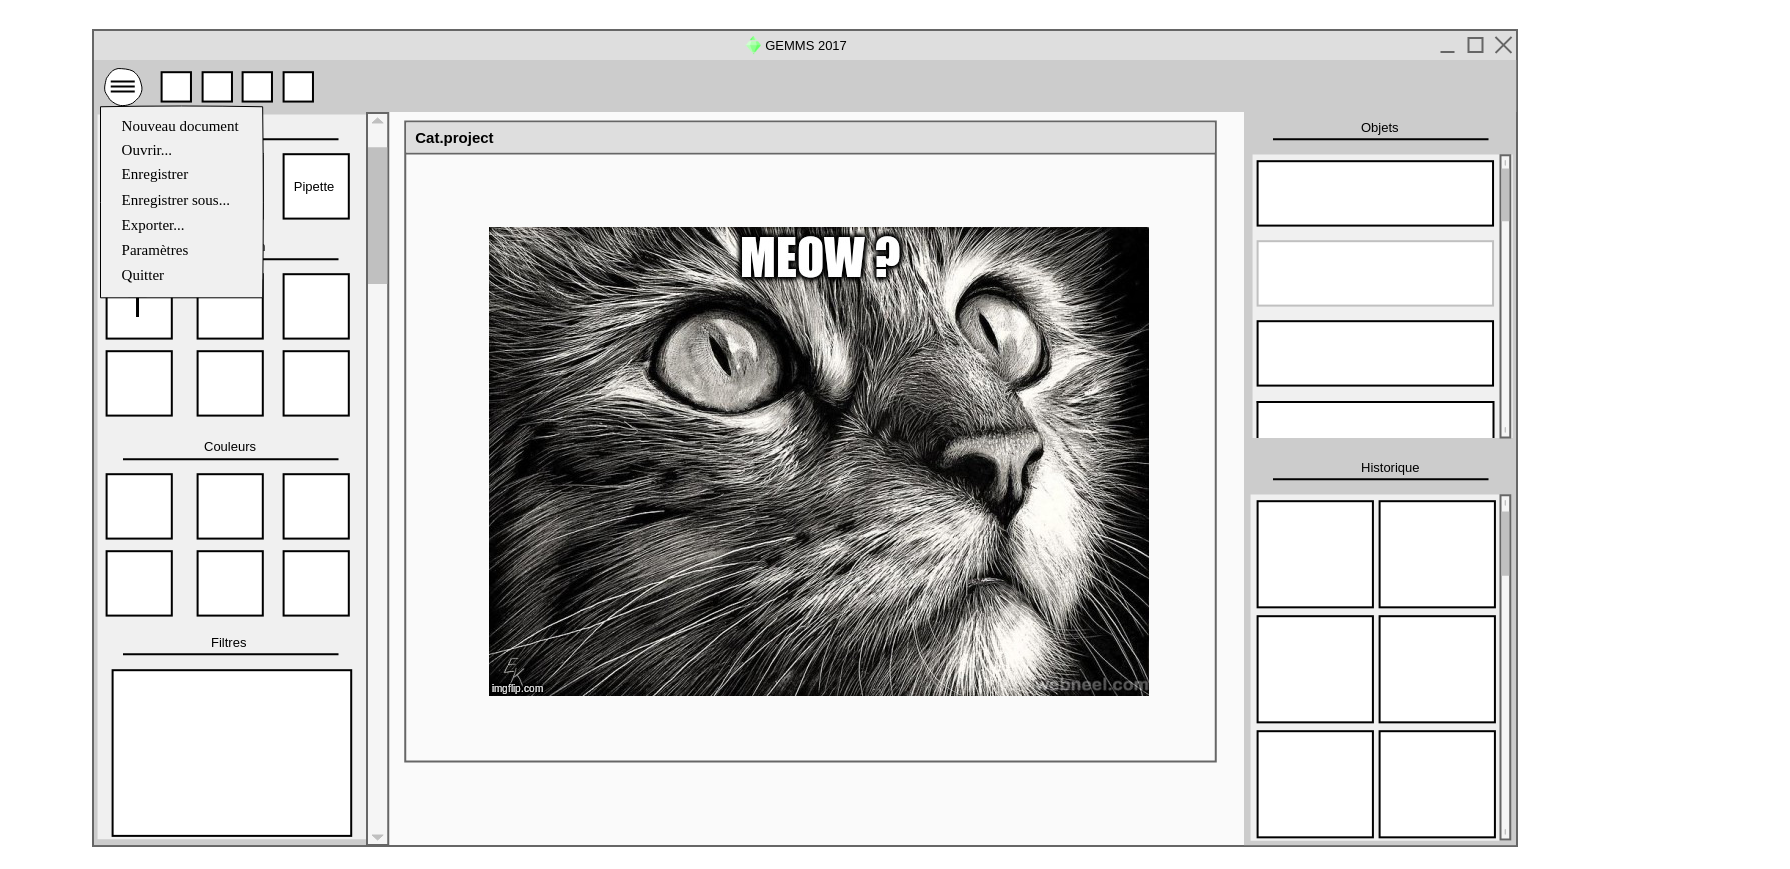
\includegraphics[scale=0.3]{menu.png}
			\caption{\label{étiquette} Menu de l'application}
		\end{figure}
	
		\begin{figure}[h!] 
			\centering
			\graphicspath{{Mockups/}}
			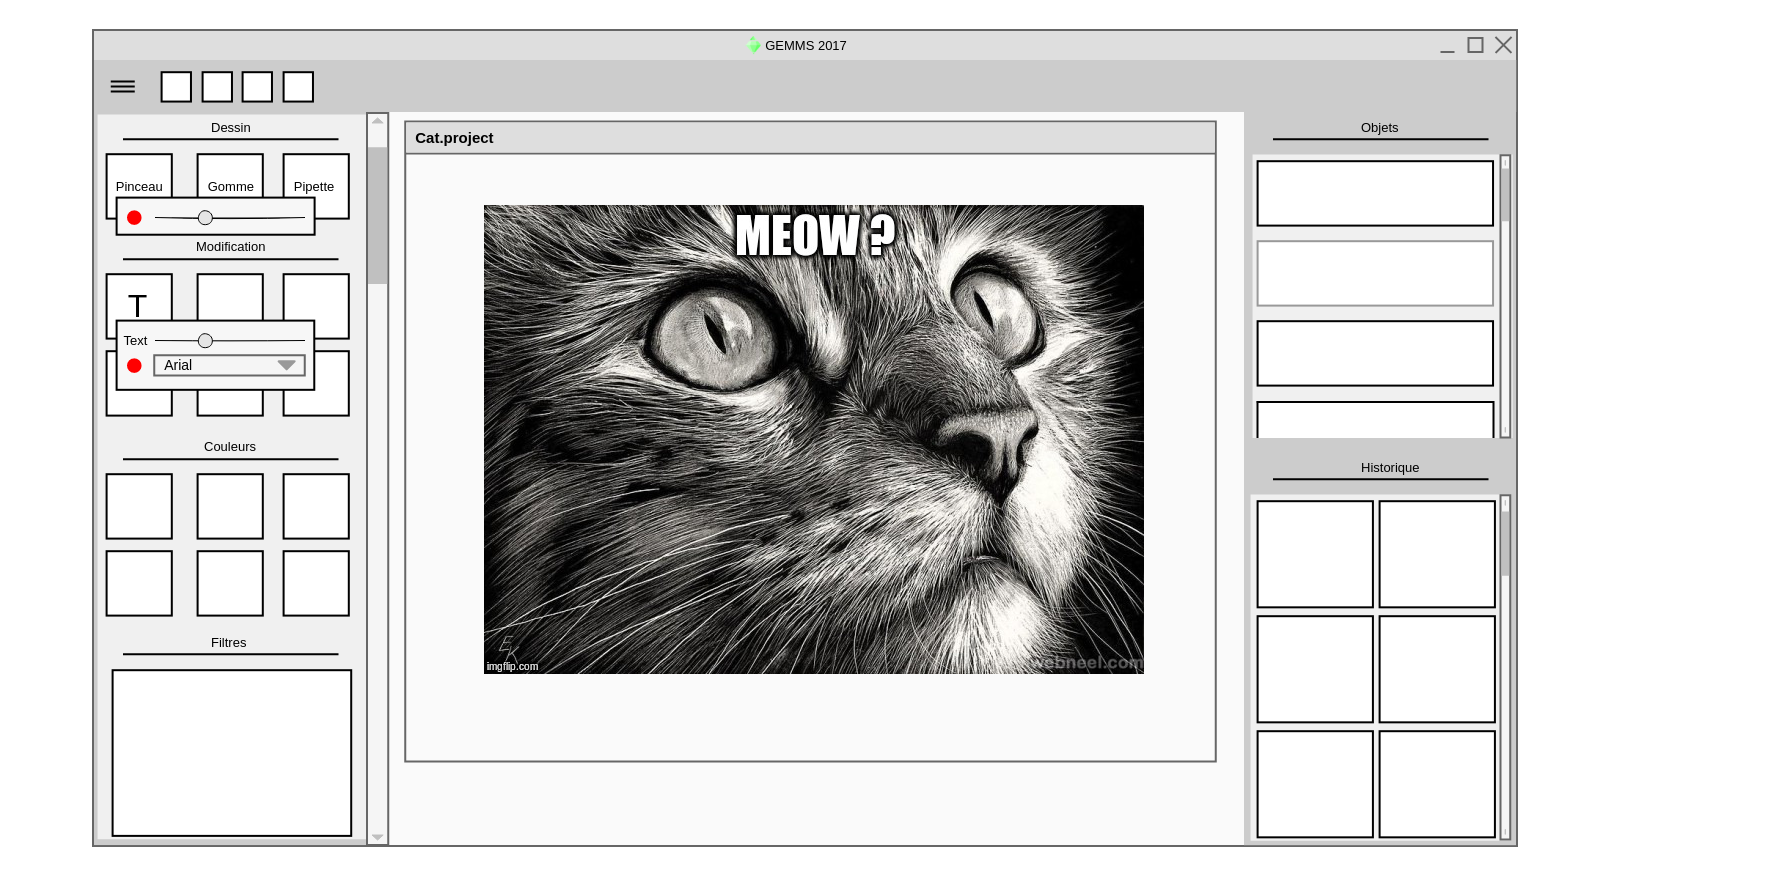
\includegraphics[scale=0.3]{tools_settings.png}
			\caption{\label{étiquette} Paramètrage des outils}
		\end{figure}
	
	
	\section{Organisation}
		\begin{tabular}{|l|l|}
			\hline
			\multicolumn{2}{|c|}{Membres de l'équipe} \\
			\hline
			Chef de projet &  Monteverde Mathieu \\ \hline
			\multirow{4}{*}{Développeur} 
			& Milani Guillaume \\
			& Kirushnapillai Sathiya \\
			& Ransome Edward \\
			& Spierer Michaël \\ \hline
		\end{tabular}
	
	\section{Planning et charge de travail}
	Ci-joint le planning Gantt ainsi qu'un schéma de la charge de travail de chacun des membres de l'équipe. On remaque que chacun d'eux travaille de façon homogène sur l'ensemble de la durée du projet.
	
\end{document}



